\chapter{Device Background}\label{cha:device_background}

Before describing measurements at the focus of this thesis, it is important to first introduce the devices we use to engineer interesting states, and the tools we use to measure them. As an overview, we use a material called GaAs/AlGaAs heterostructure, the precise layering of the semiconductors form a two-dimensional electron gas (2DEG) below the surface of the heterostructure. Voltages applied to patterened metallic gates ontop of the heterostructre can control the electrons in the 2DEG allowing for the formation of quantum point contacts (QPCs) and quantum dots  (QDs). Ohmics are used to contact the 2DEG, allowing for transport measurements through such structures. 

\section{Two-Dimensional Electron Gas (2DEG)}



\begin{figure}[ht]
  \begin{center}
%% psfrag: comment the following line if not using the psfrag package
    % \psfrag{pie makes me happy!}{$\pi$ makes me happy!}
%% includegraphics: comment the following if not using the graphicx package
    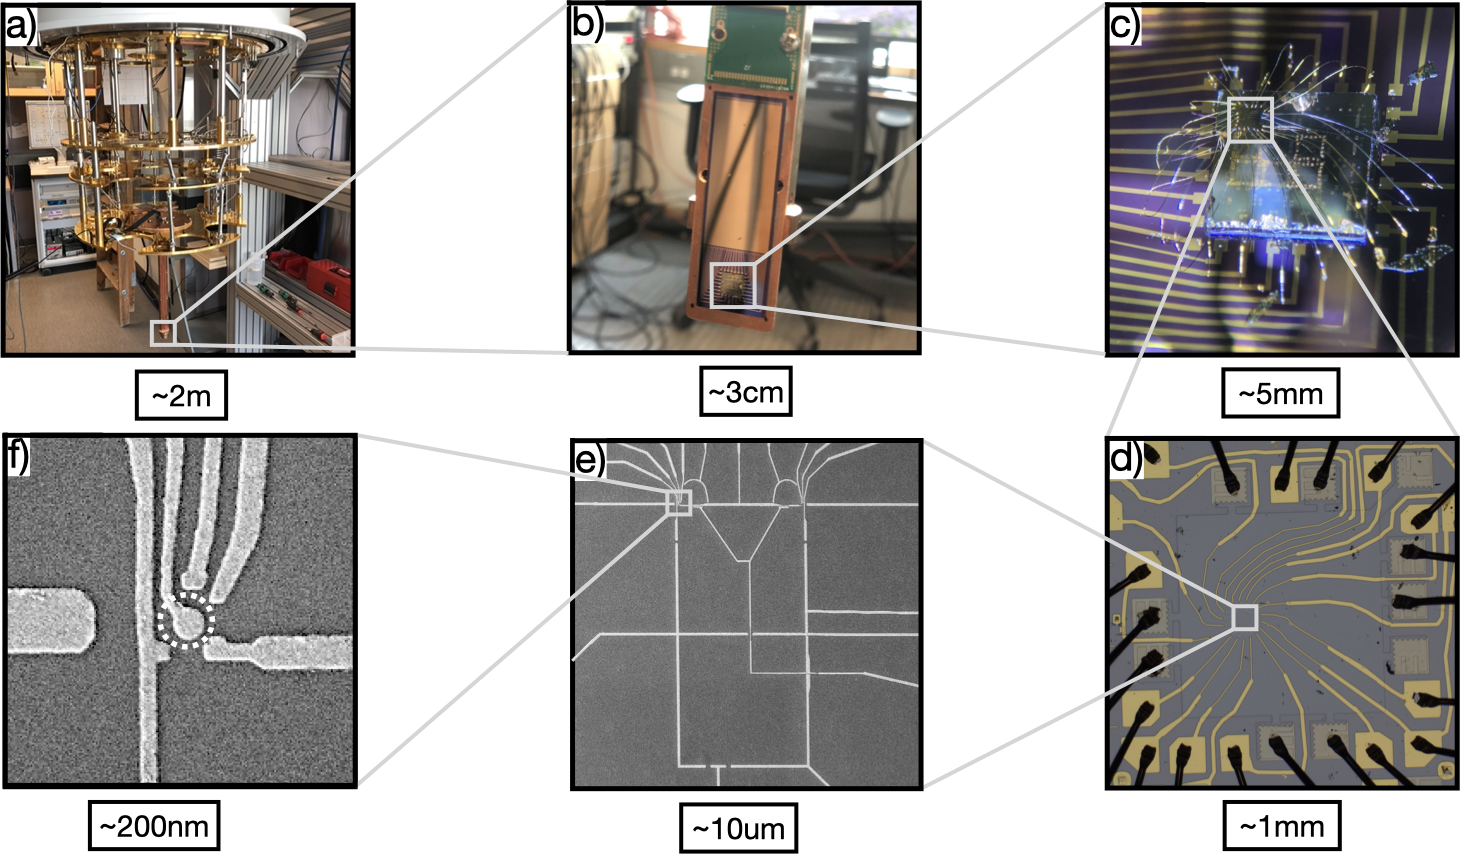
\includegraphics[width=1.0\textwidth]{figures/ch1/crop_PosterFiguresMaster.001.png}
    \caption[Two-dimensional electron gas in a GaAs/AlGaAs heterostructure]{\label{fig:ch1/2deg} 
    % For some options that work with pdf\LaTeX, please see this discussion:
    %   \url{http://tex.stackexchange.com/questions/11839}.  
    CAPTION TO BE ADDED. FIGURE TO BE CHANGED TOI HETEROSTRUCTURE.  
      }
  \end{center}
\end{figure}



The quantum point contacts (QPCs) and quantum dots (QDs) described later in this thesis are engineered in a two-dimensional electron gas (2DEG). A 2DEG can be thought of as a two dimensional plane of electrons which can move freely along the x and y direction, but are tightly confined in the z direction. The 2DEGs' in this thesis are realised in GaAs/AlGaAs heterostructures. A semiconductor heterostructure refers to a material system composed of two or more semiconductor materials with different bandgaps or lattice constants that are layered together Fig.~\ref{fig:ch1/2deg}. These layers are typically grown on top of each other using techniques such as molecular beam epitaxy (MBE). The heterostructures in this thesis are grown by Michael Manfra's lab at Purdue University [reference XXX]. 

There are two characteristics of this heterostructure which give rise to a 2DEG. Firstly, $\mathrm{Al_xGa_{1-x}As}$ has a tunable bandgap ranging from 1.42 - \qty{2.16}{eV} [REFERENCE XXX] whilst GaAs has a bandgap of \qty{1.42}{eV}. Secondly, an n-type dopant layer is sandwiched between the $\mathrm{Al_xGa_{1-x}As}$ layers. The smaller bandgap of GaAs allows the electrons from the donar atoms in the dopant layer to drop into the GaAs conduction band resulting in a triangular potential well. This triangular well contains of multiple sub-bands. The second sub-band is $\qty{\sim 150}{meV}$ above the first and will remain unoccupied as than energy gap is much greater than measurement temperatures $\qty{500}{mK}\sim\qty{43}{\mu eV}$ and source-drain bias $\qty{100}{\mu eV}$, hence, the electron gas can be considered two-dimensional.

Efforts are made to keep the heterostructure and 2DEG clean and defect free. A \qty{7}{nm} cap of GaAs is placed ontop of the heterostructure to prevent oxidation. A small lattice mis-match between the GaAs and AlGaAs layers keeps the number of boundary defects in the 2DEG plane low. The \qty{30}{nm} AlGaAs buffer layer between the 2DEG and dopants helps prevent defects near the 2DEG plane. The resulting 2DEGs' has a high mobility $\mathrm{\mu_e}~=~\qty{2.56e6}{cm^2/Vs}$ and electron density $\mathrm{n}~=~\qty{2.42e11}{cm^{-2}}$

Fabrication details on these devices `re described in Appendix [XXX]. As an overview, the heterostructure is divided into separate areas with isolated 2DEGs' by etching away the top layers of the heterostructure to remove the 2DEG. Contact to the 2DEG is made with ohmics contacts. These are made by annealing a layer of Ni-Au-Ge, the metal diffuses through the heterostructure and forms an electrical connection to the 2DEG. An insulating dielectric of \qty{10}{nm} $\mathrm{Al_2O_3}$ is deposited across the surface of the heterostructure to limit leakage from the metallic gates.  A thin layer (\qty{10}{nm}) of Au is deposited to form the inner gates which we design to form the QPCs and QDs. In a second step, a thick layer (\qty{100}{nm}) of Au is deposited (our outer gates) to connect the inner gates to square bond pads. Wire bonds are then made from chip carrier to the square bond pads which allows for connection between fridge wiring and the quantum device. 

\begin{figure}[ht]
  \begin{center}
%% psfrag: comment the following line if not using the psfrag package
    % \psfrag{pie makes me happy!}{$\pi$ makes me happy!}
%% includegraphics: comment the following if not using the graphicx package
    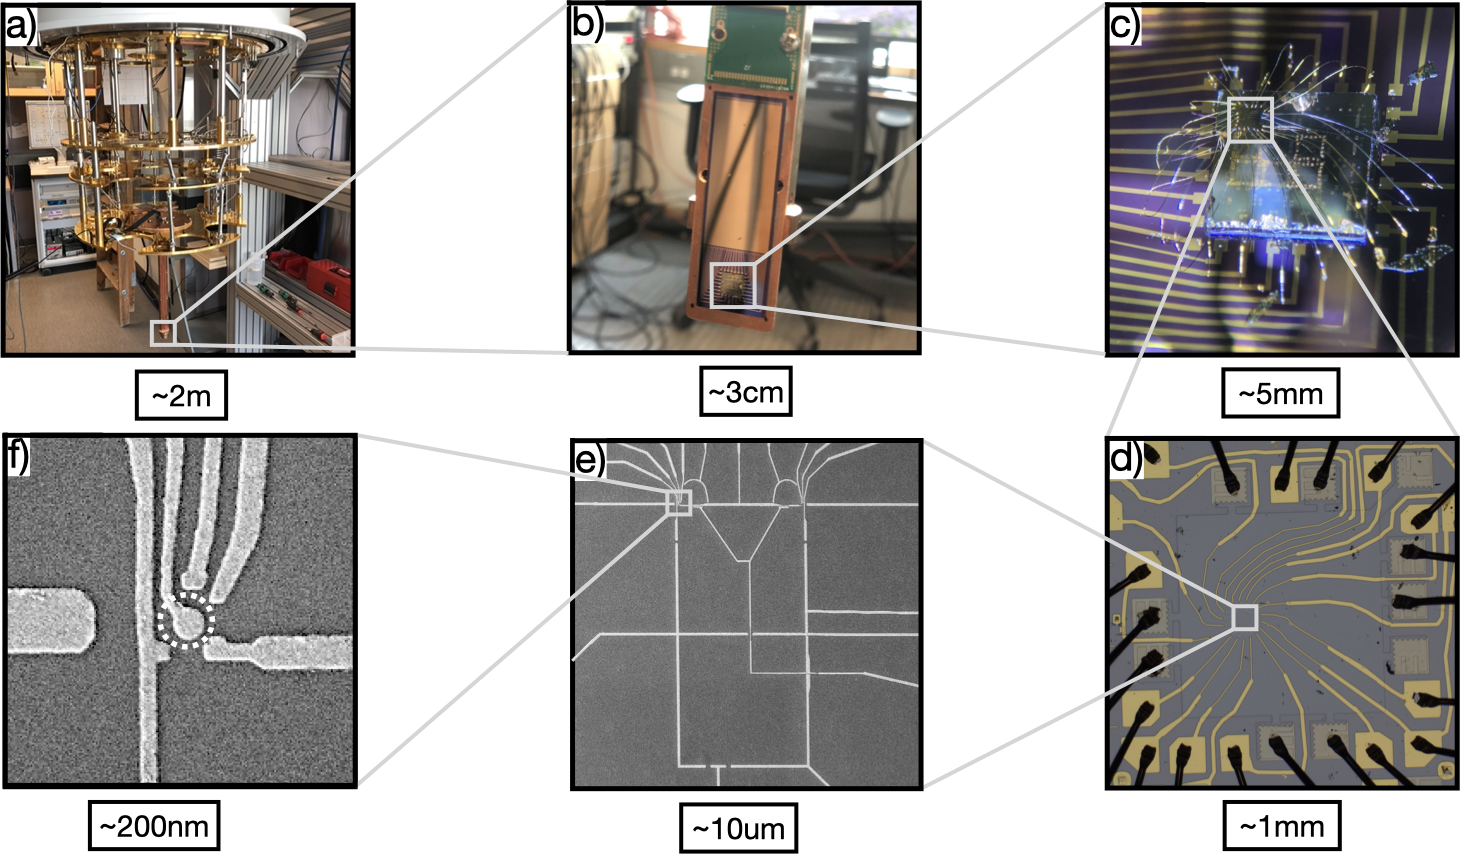
\includegraphics[width=1.0\textwidth]{figures/ch1/crop_PosterFiguresMaster.001.png}
    \caption[Dilution fridge to quantum dot scale breakdown]{\label{fig:ch1/scale_breakdown} 
    % For some options that work with pdf\LaTeX, please see this discussion:
    %   \url{http://tex.stackexchange.com/questions/11839}.  
    Showing the various scales to connect how macro changes affect the nano. (\textbf{a}) A photograph of the Au plated cold plates in our dilution refridgerator. The lowest plate is called the mixing chamber and can reach \qty{7}{mK}. (\textbf{b}) A photograph of the Si chip carrier, onto which the heterostructure is stuck to. (\textbf{c}) An optical microscope image of the heterostructure stuck to the chip carrier. The thin wires are Al wire bonds which connect the device fabricated on the heterostructure to the fridge wires. (\textbf{d}) An optical microscope image of a single mesa on the heterostructure. A mesa is an isolated area of the heterostructure where we fabricate new designs. The black lines around the outside are the wire bonds and the bright Au are the thick (\qty{100}{nm}) 'outer gates' which connect to the thin (\qty{10}{nm}) 'inner gates'. (\textbf{d}) A scanning electron micrograph (SEM) of the inner gates. The mean free path of the electrons is of order \qty{3}{\mu m}.  (\textbf{d}) An SEM image zoom-in on the quantum dot. By carefully tuning the voltages on the inner gates, we can create an isolated puddle of electrons, typically with total occupation 0 - 10.  
      }
  \end{center}
\end{figure}




\section{Quantum Point Contact (QPC)}


\begin{figure}[ht]
  \begin{center}
%% includegraphics: comment the following if not using the graphicx package
    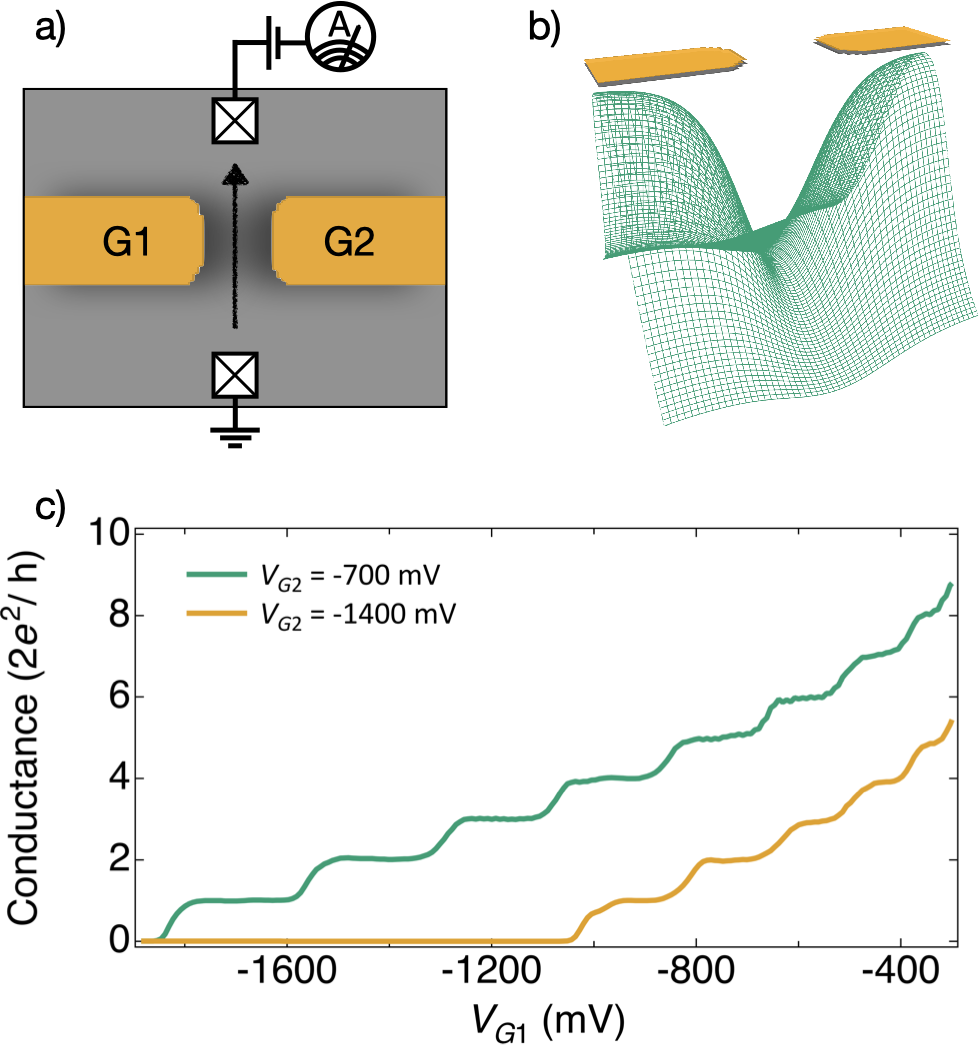
\includegraphics[width=0.9\textwidth]{figures/ch1/crop_PosterFiguresMaster.002.png}
    \caption[Conductance through a quantum point contact]{\label{fig:ch1/qpc_intro} 
    % For some options that work with pdf\LaTeX, please see this discussion:
    %   \url{http://tex.stackexchange.com/questions/11839}.  
    (\textbf{a}) A graphic representation from a top-down view of a quantum point contact (QPC). The gold fingers are the metallic gates where negative voltages can be applied to. The grey is where the electrons in the 2DEG can go dependant on the amount of negative voltage applied to the gates. The crossed squares are ohmic contacts to the 2DEG so that bias can be applied and the conductance through the QPC is measured. (\textbf{b}) is a representation of the electric potential the electrons see in the 2DEG due to negative voltage applied to the gates. With sufficient negative voltages applied to the gates, the electrons cannot overcome the potential barrier under the gate and flow through the middle. (\textbf{c}) is a measurement showing the quantised conductance through a QPC as the voltage on G1 becomes more negative. The voltage on the gates can be made negative enough so that electrons cannot tunnel across the potential barrier and hence we measure 0 conductance. 
      }
  \end{center}
\end{figure}



In this thesis a quantum point contact (QPC) is one-dimensional channel connected to a source and drain reservoir Fig.~\ref{fig:ch1/qpc_intro}. A one-dimensional channel in the 2DEG is engineered by putting sufficient negative voltage on metal gates deposited on the surface of the heterostructure. By applying a potential bias between the ohmics a current will flow. The more negative the voltage on the gate, the higher the potential barrier is for the electrons in the 2DEG. A large enough potential barrier can stop the electrons flowing underneath the gate (called 'depletion'), however, they can still flow between the gates. It normally requires a more negative voltage to stop electrons flowing between the gates (called 'pinch-off'). A QPC length is the length of the one-dimensional channel and the width is the empty space between gates. In our devices, QPCs' have lengths 50~-~\qty{350}{nm} and widths 100~-~\qty{350}{nm}.

If the width of the QPC is comparable to the Fermi wavelength, the electrons will be quantised in the x-direction and free to move in the y-direction. The confining potential in the x-direction can be modelled as a parabolic potential and hence the allowed 1d sub-bands will resemble solutions to the harmonic oscillator Fig.~\ref{fig:ch1/qpc_intro}\textbf{b}. In the absence of a magnetic field, each occupied sub-band contributes $\mathrm{2e^2/h}$ to the conductance. The $2$ comes from the spin degeneracy of the electrons which can be lifted with magnetic field. When measuring the conductance through a QPC as it is pinched off Fig.~\ref{fig:ch1/qpc_intro}\textbf{c} we see the quantised conductance as plateaus at integer values of $\mathrm{2e^2/h}$. At zero temperature the conductance would increase in sharp steps but this is smeared out by temperature in a real measurement.

In our devices, QPCs are used to form tunable tunnel barriers between a quantum dot and a reservoir (described in the next section) and charge sensors which are used to measure the charge around a quantum dot. 



\section{Quantum Dot (QD)}

In this thesis a quantum dot (QD) is zero-dimensional structure, it can be formed by connecting a potential well to source and drain reservoirs through tunnel barriers. The tunnel barriers are formed by QPCs. Similar to a QPC, the potential well is formed by applying negative voltages to gates to confine a small region in the 2DEG Fig.~\ref{fig:ch1/dot_intro}\textbf{a}. The energy level spacing of the QD are determine by two 

\begin{figure}[ht]
  \begin{center}
%% includegraphics: comment the following if not using the graphicx package
    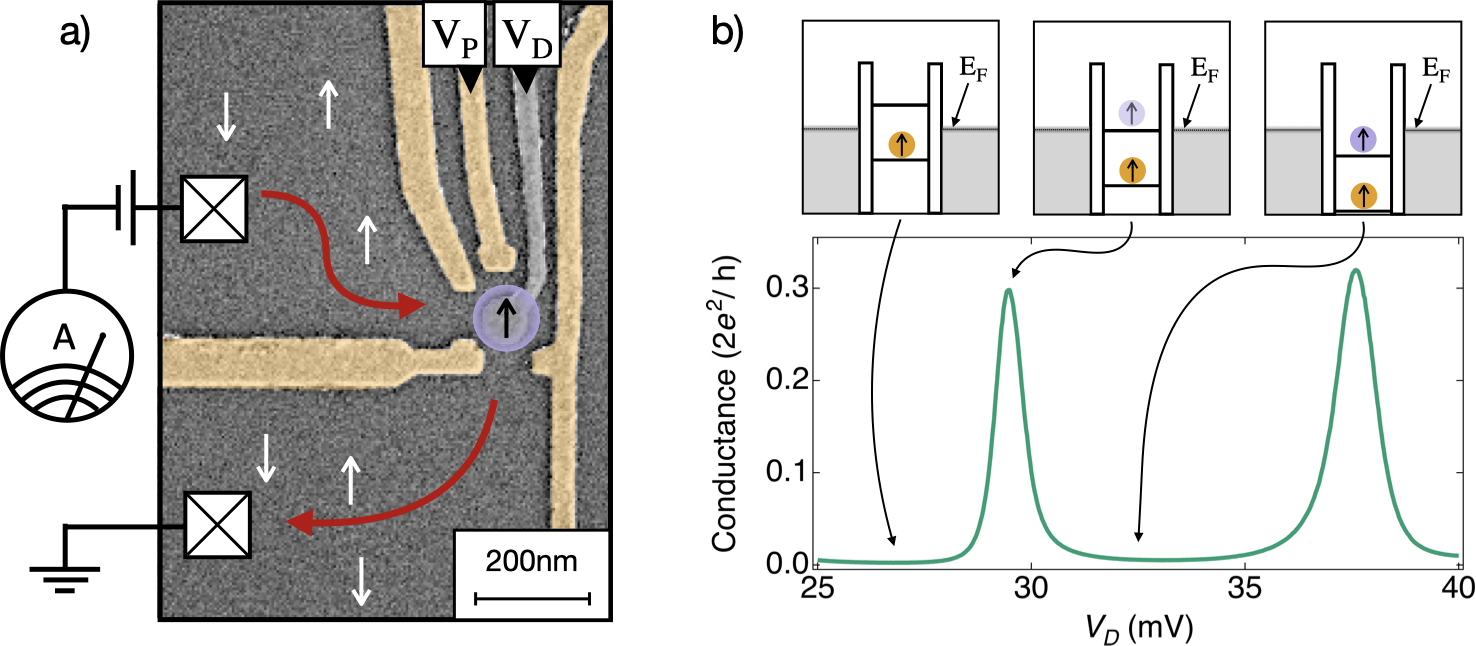
\includegraphics[width=1.0\textwidth]{figures/ch1/crop_PosterFiguresMaster.003.png}
    \caption[Conductance through a quantum dot]{\label{fig:ch1/dot_intro} 
    % For some options that work with pdf\LaTeX, please see this discussion:
    %   \url{http://tex.stackexchange.com/questions/11839}.  
    (\textbf{a}) an SEM image of the gates used to define a quantum dot. The gold coloured gates indicate sufficient negative potential is applied so that the 2DEG below is depleted. The gates V\textsubscript{P} or V\textsubscript{D} have the biggest effect on dot energy without changing other energies. The crossed are ohmic contacts which contact the 2DEG. By applying a small bias we measure the conductance through the quantum dot. (\textbf{b}) are Coulomb blockade energy diagrams illustrating how the conductance varies as an electron enters the quantum dot. The grey boxes represent the continuous energy level of electrons in the leads. The white rectangles represent tunnel barriers into and out-of the quantum dot. The rate of tunneling is described by the parameter $\Gamma$, the wider (narrower) the barrier, the smaller (larger) the rate of tunneling. (\textbf{c}) is a measurement showing the conductance through a quantum dot as a single electron (in purple) is added. From left to right: Electrons in the leads cannot tunnel into the quantum dot as there is no available energy level and hence we measure zero conductance. As V\textsubscript{D} is made less negative, the dot energy lowers and electrons can tunnel into the dot and back out. We measure a maximum in conductance when the dot energy is aligned with the leads. Once the dot energy falls below the level of the leads there is again no available energy level and the dot is insulating. 
      }
  \end{center}
\end{figure}


\begin{figure}[ht]
  \begin{center}
%% includegraphics: comment the following if not using the graphicx package
    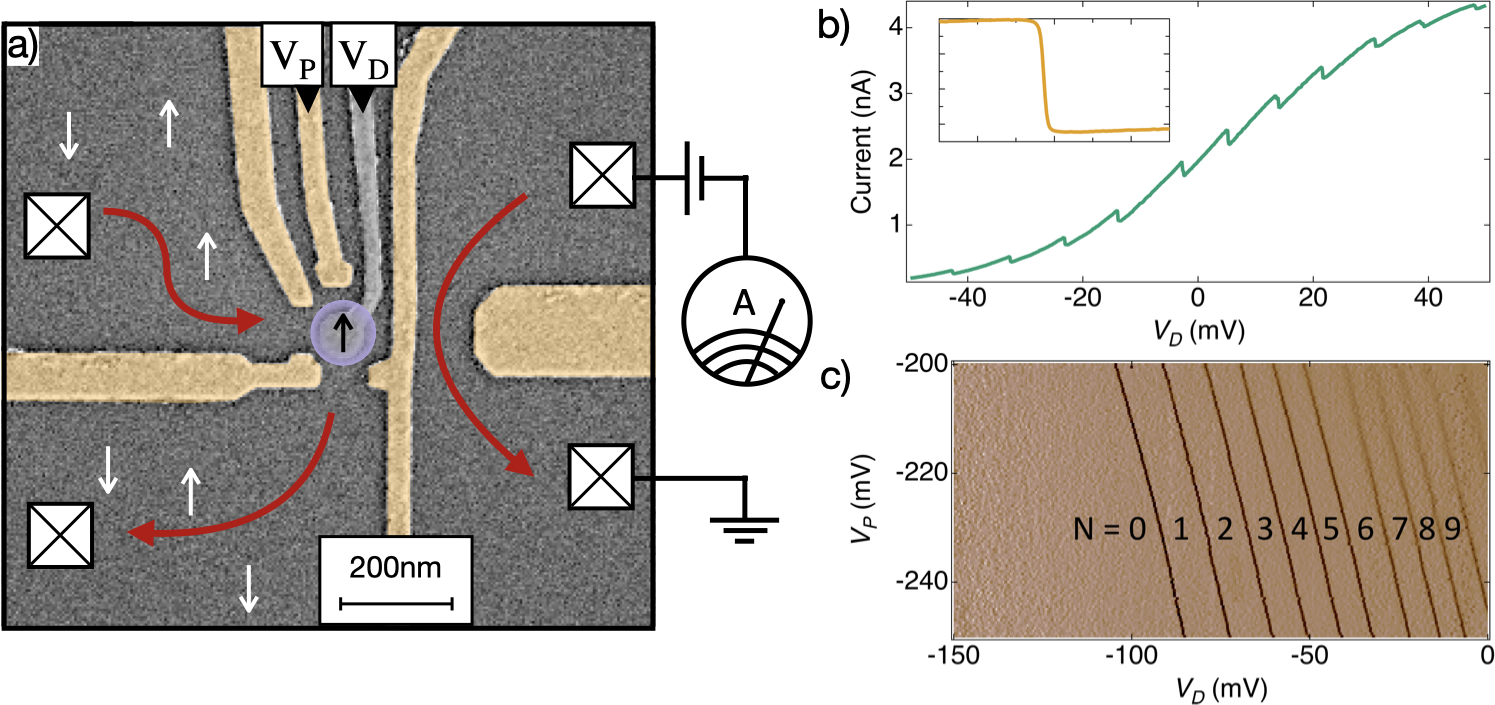
\includegraphics[width=1.0\textwidth]{figures/ch1/crop_PosterFiguresMaster.004.png}
    \caption[Charge sensing a quantum dot]{\label{fig:ch1/ct_intro} 
    % For some options that work with pdf\LaTeX, please see this discussion:
    %   \url{http://tex.stackexchange.com/questions/11839}.  
    (\textbf{a}) An SEM image of the gates used to define a quantum dot. The gold coloured gates indicate sufficient negative potential is applied so that the 2DEG below is depleted. The gates V\textsubscript{P} or V\textsubscript{D} have the biggest effect on dot energy without changing other energies. The crossed are ohmic contacts which contact the 2DEG. V\textsubscript{CSQ} is used to form a QPC near the quantum dot. By setting up the QPC on a steep slope the current through the QPC is sensitive to nearby changes in charge. (\textbf{b}) measuring the current across the charge sensing QPC. As V\textsubscript{D} becomes less negative the current through the QPC increases. The downward jumps in current are a result of the negative repulsion from electrons entering the quantum dot. The subfigure (yellow) shows a zoomed in scan over one of these transitions. (\textbf{c}) A 2d map showing how the occupation of the quantum dot changes as a function of V\textsubscript{P} and V\textsubscript{D}. The data is the differentiated current through the charge sensor. The differentiated steep slopes of the charge transitions show up as sharp peak which is useful for locating charge transitions when there is a large change in background current. 
      }
  \end{center}
\end{figure}



\begin{figure}[ht]
  \begin{center}
%% includegraphics: comment the following if not using the graphicx package
    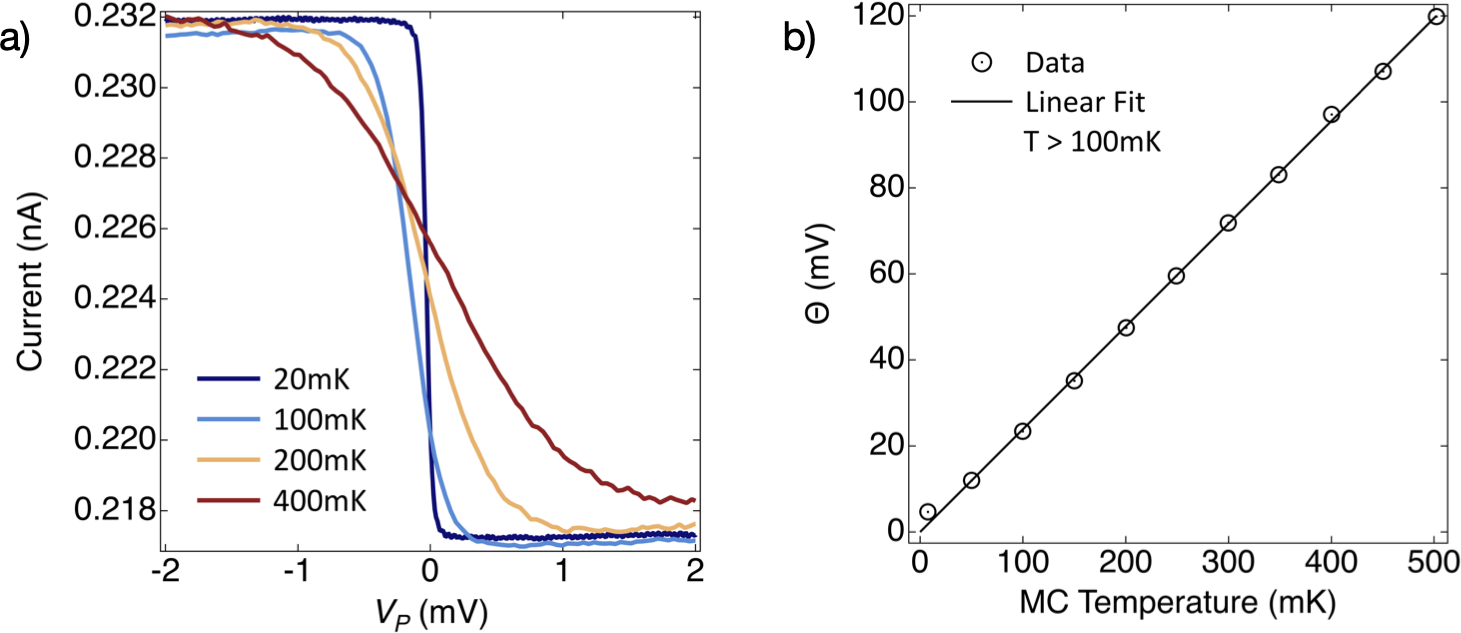
\includegraphics[width=1.0\textwidth]{figures/ch1/crop_PosterFiguresMaster.005.png}
    \caption[Calculating the electron temperature]{\label{fig:ch1/electron_temp} 
    % For some options that work with pdf\LaTeX, please see this discussion:
    %   \url{http://tex.stackexchange.com/questions/11839}.  
    (\textbf{a}) A weakly coupled charge transition measured at different fridge temperatures. The broadening of a weakly coupled charge transition is linearly proportional to its temperature. (\textbf{b}) A plot of the calculated broadening ($\Theta$) of the charge transition at different fridge temperatures. At fridge temperatures \qty{>100}{mK}, the increase in the charge transition broadening is linear. This indicates the electrons are well thermalised to the fridge. A linear fit to fridge temperatures \qty{>100}{mK} is extrapolated to base temperature to calculate the temperature of the electrons given the measure broadening. 
      }
  \end{center}
\end{figure}


Here is a reference to the above figure ~\ref{fig:ch1/scale_breakdown}